\documentclass[aspectratio=169]{beamer}
\usepackage{color,amsmath}
\usepackage{subfigure}
\usepackage{booktabs}
\usepackage{framed}
\usepackage{comment}

%%%%%%%%%%%%%%%%%%%%%%%%%%
\title[]{Survey research in the digital age}
\author[]{Matthew J. Salganik\\Department of Sociology\\Princeton University}
\date[]{Summer Institutes in Computational Social Science\\June 20, 2019
\vfill
\begin{flushleft}
{\scriptsize
The Summer Institutes in Computational Social Science is supported by grants from the Russell Sage Foundation and the Alfred P. Sloan Foundation.}
\end{flushleft}
\begin{flushright}
\vfill

\includegraphics[width=0.1\textwidth]{figures/cc-by.png}
\end{flushright}
}
\begin{document}
%%%%%%%%%%%%%%%%%%%%%%%%%%
\frame{\titlepage}
%%%%%%%%%%%%%%%%%%%%%%%%%%
\begin{frame}

\begin{center}
\begin{tabular}{ccc}
\onslide<1-3>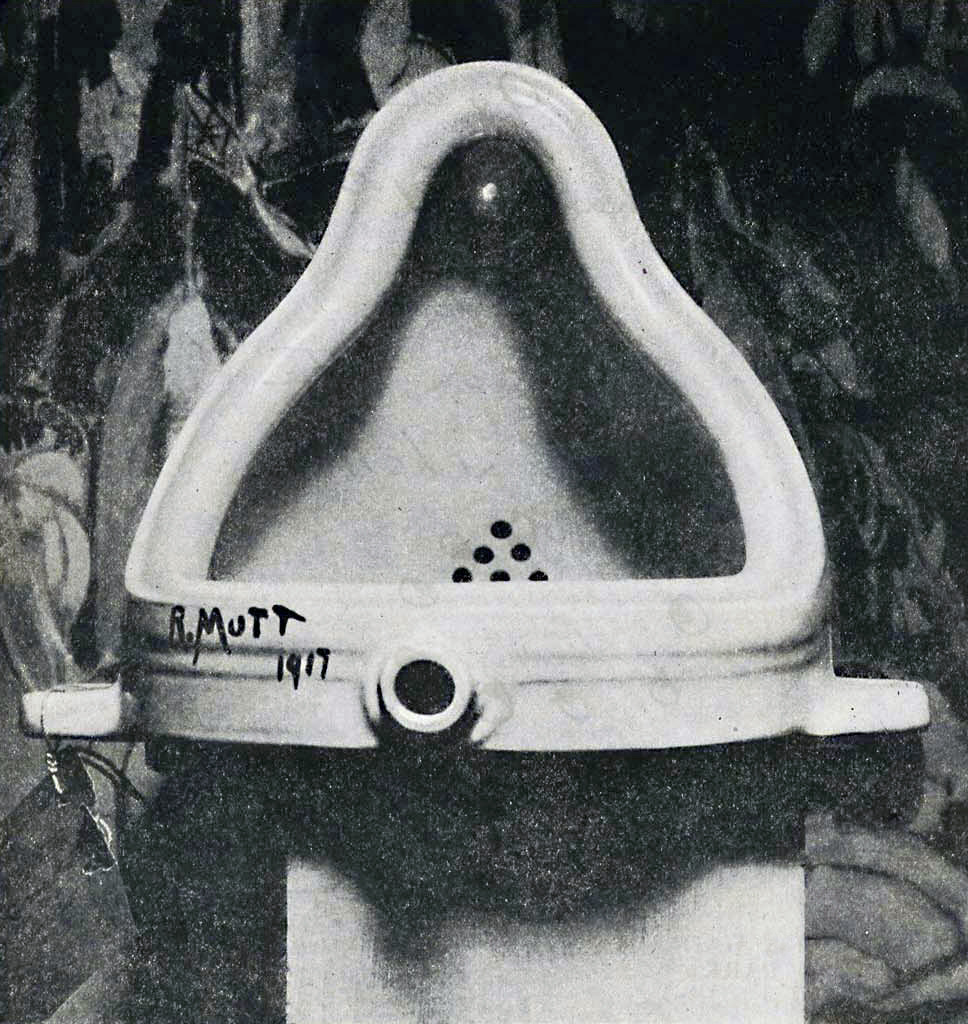
\includegraphics[width=0.30\textwidth]{figures/duchamp_fountain} & \phantom{12345} & \onslide<2-3>{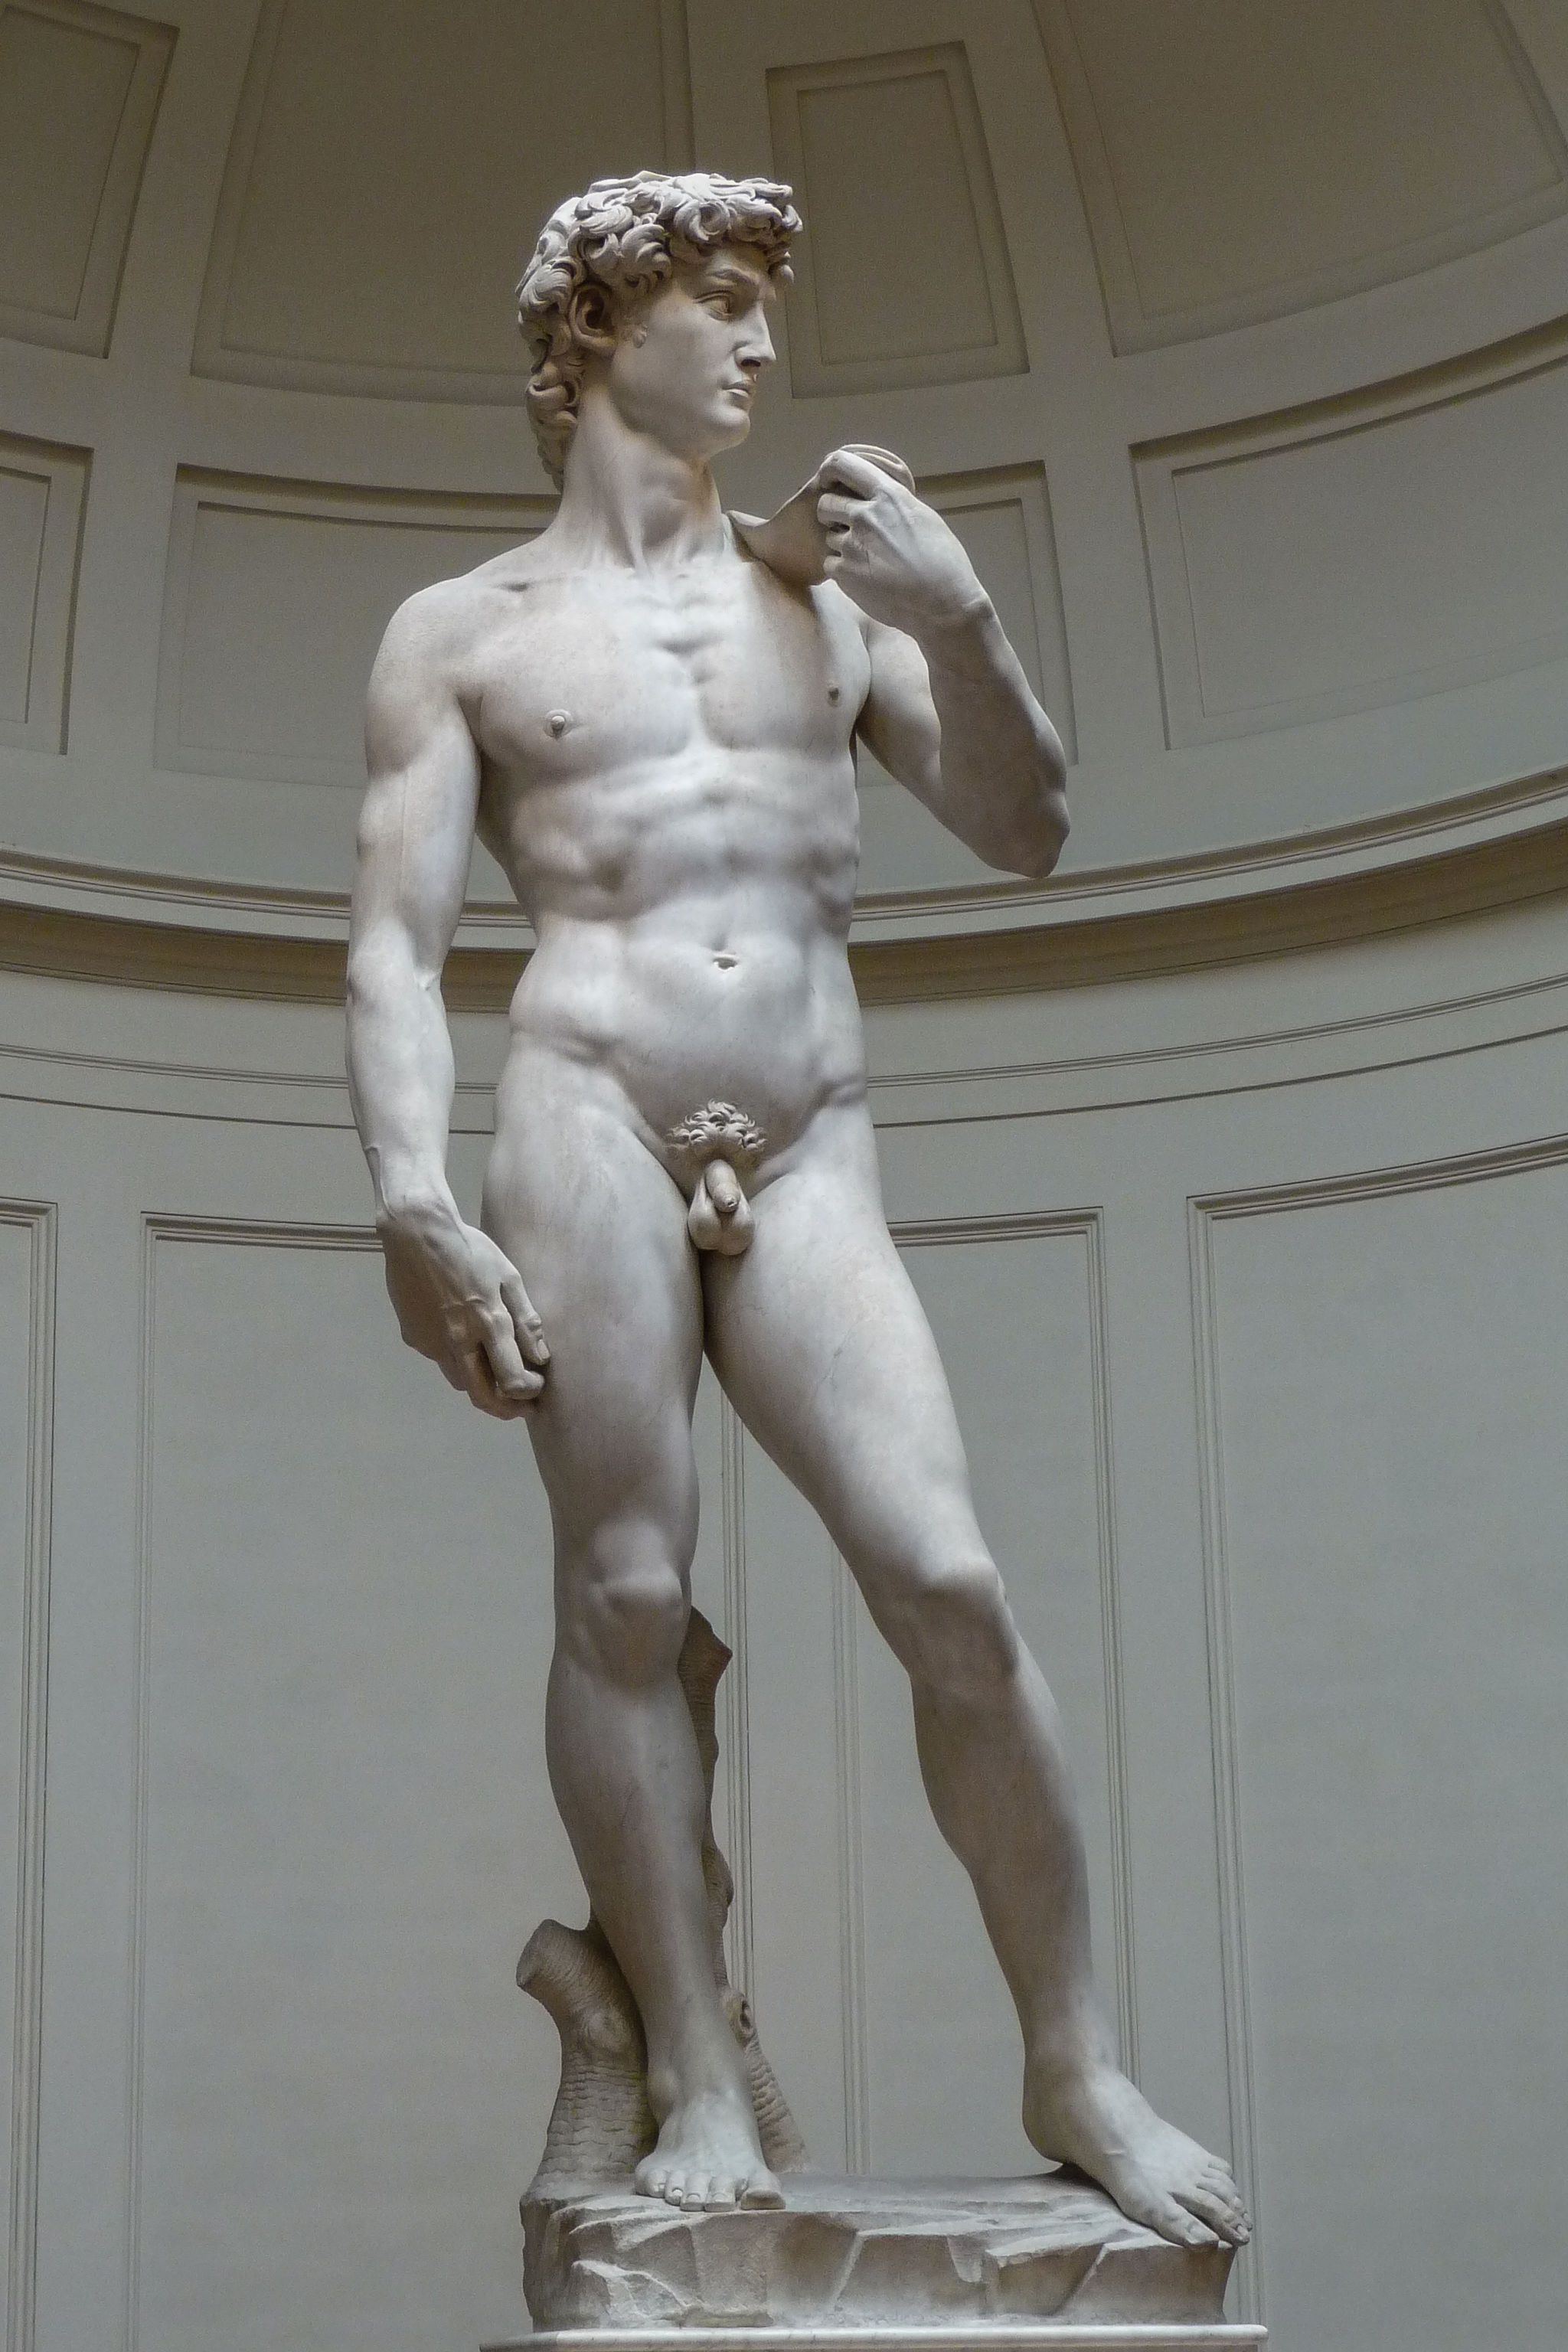
\includegraphics[width=0.30\textwidth]{figures/michelangelo_david}} \\
\onslide<3>{\LARGE{readymades}} &  & \onslide<3>{\LARGE{custommades}}
\end{tabular}
\end{center}

\vfill
\onslide<3>{
\TINY{\url{https://commons.wikimedia.org/wiki/File:Duchamp_Fountaine.jpg}}\\
\TINY{\url{https://commons.wikimedia.org/wiki/File:\%27David\%27_by_Michelangelo_JBU0001.JPG}}}

\end{frame}
%%%%%%%%%%%%%%%%%%%%%%%%%%
\begin{frame}

Schedule for today: 

\end{frame}
%%%%%%%%%%%%%%%%%%%%%%%%%%%
\begin{frame}

A few notes on my teaching:
\begin{itemize}
\item Anti-status quo bias
\pause
\item Anti-formality bias (formality is important, but just not right now)
\pause
\item Very brief to leave time for the activity
\pause
\item More information in Chapter 3 of \textit{Bit by Bit: Social Research in the Digital Age}: \url{https://www.bitbybitbook.com/en/1st-ed/asking-questions/}
\end{itemize}

\end{frame}
%%%%%%%%%%%%%%%%%%%%%%%%%
\begin{frame}

\begin{center}
\LARGE{Why should I care about surveys?}
\end{center}

\end{frame}
%%%%%%%%%%%%%%%%%%%%%%%%%%%%%
\begin{frame}

\begin{center}
\LARGE{Why should I care about surveys\\in the age of big data?}
\end{center}

\end{frame}
%%%%%%%%%%%%%%%%%%%%%%%%%%%%%
\begin{frame}

We will always need to ask
\begin{itemize}
\item limitations of big data (fubu vs. nufu-nubu)
\pause
\item internal states vs. external states
\pause
\item inaccessibility of big data
\end{itemize}

\pause
\vfill
But how we are going to ask is going to change
\end{frame}
%%%%%%%%%%%%%%%%%%%%%%%%%%%
\begin{frame}

\begin{center}
\begin{tabular}{ l c c}
           & Sampling& Interviews \\
\hline
1st era & Area probability & Face-to-face \\
\pause
2nd era & Random digital dial probability & Telephone \\
\pause
3rd era & \pause Non-probability & Computer-administered  \\
\end{tabular}
\end{center}

\end{frame}
%%%%%%%%%%%%%%%%%%%%%%%%%%%
\begin{frame}

\begin{center}
\small{
\begin{tabular}{ l c c c}
           & Sampling & Interviews & Data environment\\
\hline
1st era & Area probability & Face-to-face & Stand-alone \\
2nd era & \parbox[t]{3cm}{\centering Random digital dial\\probability} & Telephone & Stand-alone \\
3rd era & Non-probability & Computer-administered  & Linked \\
\end{tabular}
}
\end{center}

\end{frame}
%%%%%%%%%%%%%%%%%%%%%%%%%%%
\begin{frame}

\begin{center}
\small{
\begin{tabular}{ l c c c}
           & Sampling & Interviews & Data environment\\
\hline
1st era & Area probability & Face-to-face & Stand-alone \\
2nd era & \parbox[t]{3cm}{\centering Random digital dial\\probability} & Telephone & Stand-alone \\
\textcolor{blue}{3rd era} & \textcolor{blue}{Non-probability} & \textcolor{blue}{Computer-administered}  & \textcolor{blue}{Linked} \\
\end{tabular}
}
\end{center}

\end{frame}
%%%%%%%%%%%%%%%%%%%%%%%%%%%
\begin{frame}

\begin{center}
Total survey error framework
\end{center}

\pause 

\begin{columns}[T]

\begin{column}{0.48\textwidth}

{\Large Who we ask} (representation)\\
\begin{itemize}
\item sampling error
\item coverage errors
\item non-response error
\end{itemize}
\end{column}


\begin{column}{0.48\textwidth}
{\Large How we ask} (measurement)\\
\begin{itemize}
\item question wording
\item question ordering
\item social desirability bias
\end{itemize}
\end{column}

\end{columns}

\end{frame}
%%%%%%%%%%%%%%%%%%%%%%%%%%%
\begin{frame}

\begin{center}
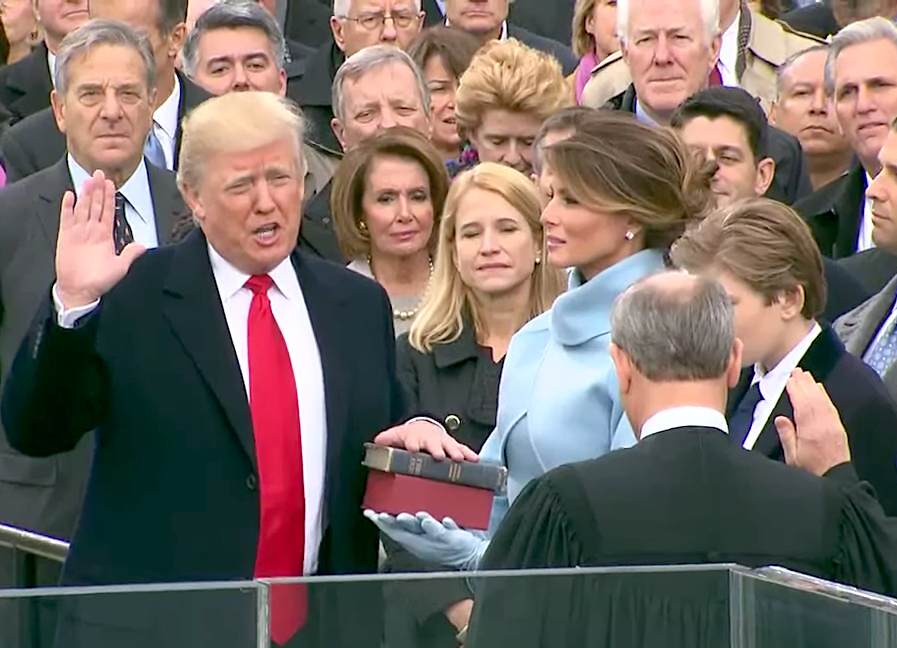
\includegraphics[width=0.6\textwidth]{figures/trump_oath}
\end{center}

\vfill
\tiny{\textcolor{blue}{\url{https://commons.wikimedia.org/wiki/File:Donald_Trump_taking_his_Oath_of_Office.png}}}

\end{frame}
%%%%%%%%%%%%%%%%%%%%%%%%%%
\begin{frame}

\begin{center}
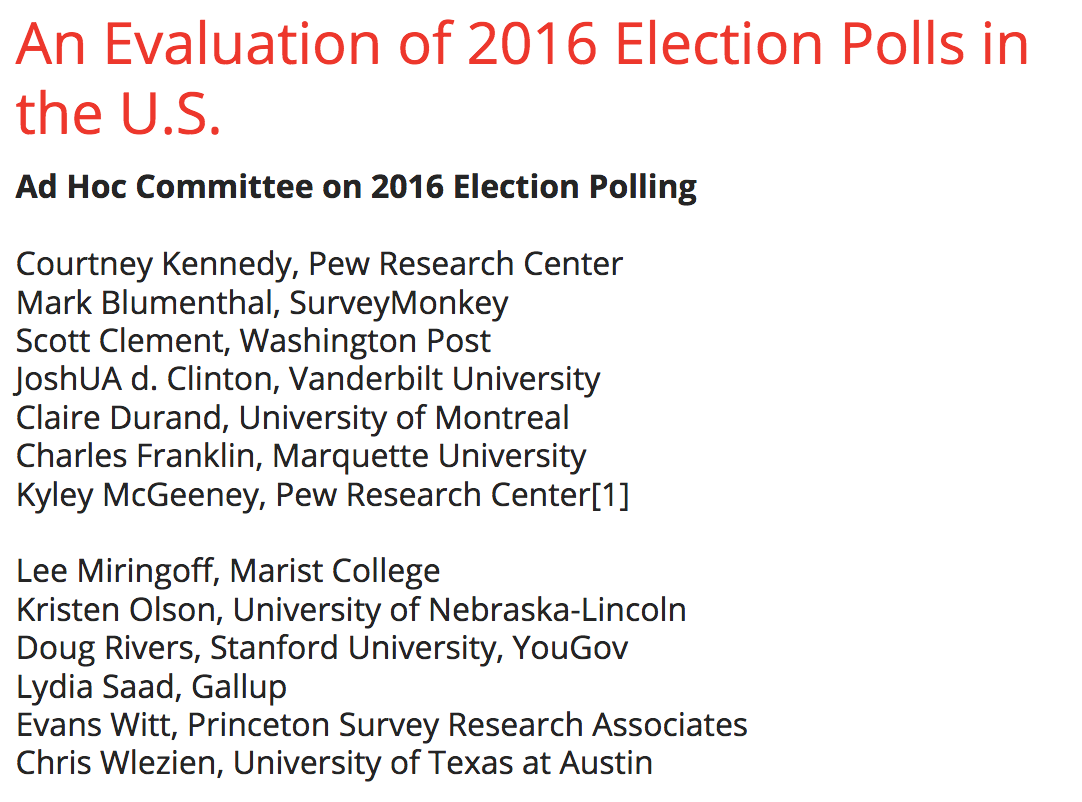
\includegraphics[width=0.5\textwidth]{figures/aapor_2016_election_evaluation}
\end{center}

\vfill
\tiny{\url{http://www.aapor.org/Education-Resources/Reports/An-Evaluation-of-2016-Election-Polls-in-the-U-S.aspx}}

\end{frame}
%%%%%%%%%%%%%%%%%%%%%%%%%%%
\begin{frame}
\begin{columns}[T]

\begin{column}{0.48\textwidth}
\textcolor{blue}{
{\Large Who we ask} (representation)}\\
\begin{itemize}
\item sampling error
\item coverage errors
\item non-response error
\end{itemize}
\end{column}


\begin{column}{0.48\textwidth}
{\Large How we ask} (measurement)\\
\begin{itemize}
\item question wording
\item question ordering
\item social desirability bias
\end{itemize}
\end{column}

\end{columns}

\end{frame}
%%%%%%%%%%%%%%%%%%%%%%%%%%%
\begin{frame}
\begin{columns}[T]

\begin{column}{0.48\textwidth}

{\Large Who we ask} (representation)\\
\begin{itemize}
\item sampling error
\item coverage errors
\item non-response error
\end{itemize}
\end{column}

\begin{column}{0.48\textwidth}
\textcolor{blue}{{\Large How we ask} (measurement)}\\
\begin{itemize}
\item question wording
\item question ordering
\item social desirability bias
\end{itemize}
\end{column}
\end{columns}

\end{frame}
%%%%%%%%%%%%%%%%%%%%%%%%%%%
\begin{frame}

\begin{center}
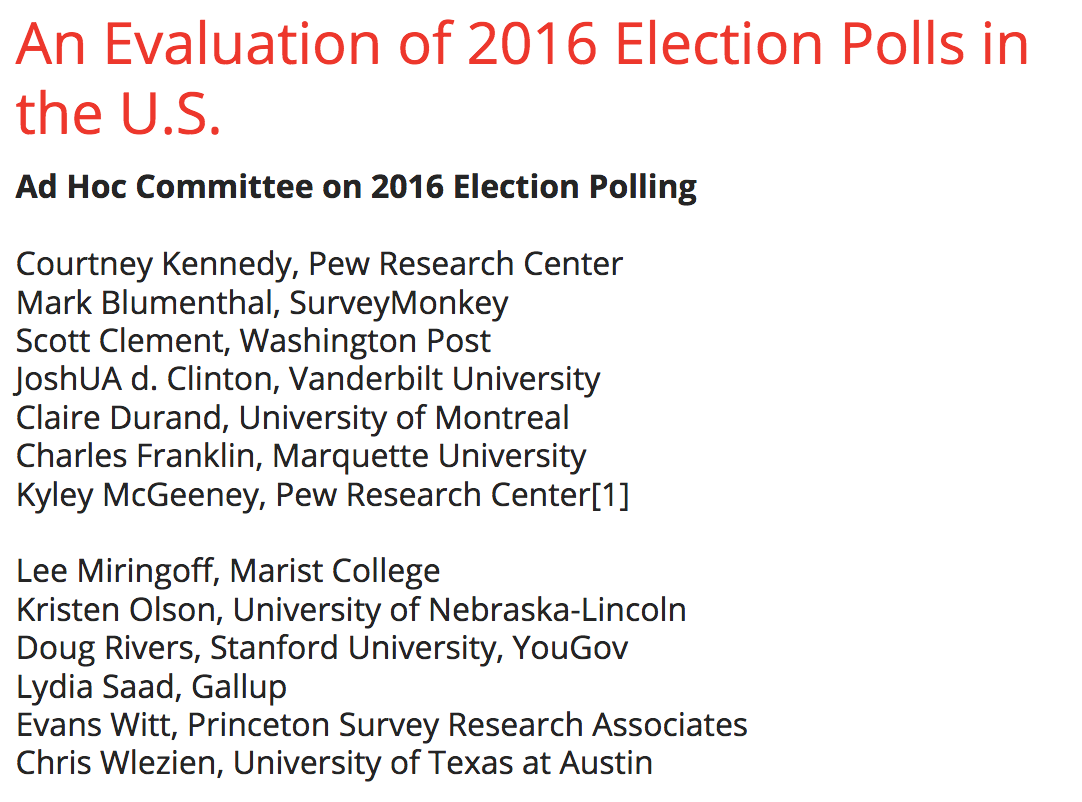
\includegraphics[width=0.5\textwidth]{figures/aapor_2016_election_evaluation}
\end{center}

\vfill
\tiny{\url{http://www.aapor.org/Education-Resources/Reports/An-Evaluation-of-2016-Election-Polls-in-the-U-S.aspx}}

\end{frame}
%%%%%%%%%%%%%%%%%%%%%%%%%%%
\begin{frame}

\begin{itemize}
\item National polls were generally correct and accurate by historical standards.
\pause
\item State-level polls showed a competitive, uncertain contest  . . . 
\pause
\item  . . . but clearly under-estimated Trump's support in the Upper Midwest.
\end{itemize}

\end{frame}
%%%%%%%%%%%%%%%%%%%%%%%%%%%%
\begin{frame}

``There are a number of reasons as to why polls under-estimated support for Trump. The explanations for which we found the most evidence are:''
\begin{itemize}
\item ``Real change in vote preference during the final week or so of the campaign''
\pause
\item ``Adjusting for over-representation of college graduates was critical, but many polls did not do it''
\pause
\item ``Some Trump voters who participated in pre-election polls did not reveal themselves as Trump voters until after the election, and they outnumbered late-revealing Clinton voters''
\end{itemize}

\vfill

Full report: \url{http://www.aapor.org/Education-Resources/Reports/An-Evaluation-of-2016-Election-Polls-in-the-U-S.aspx}

\end{frame}
%%%%%%%%%%%%%%%%%%%%%%%%%%%%%%
\begin{frame}

Wrapping up:
\pause
\begin{itemize}
\item Total survey error framework helps us organize all the things that can go wrong
\pause
\item Total survey error framework also helps us think about how digital age can create new opportunities (who to ask and how to ask)
\pause 
\item To learn more: \href{https://www.amazon.com/Survey-Methodology-Robert-M-Groves/dp/0470465468}{Groves et al (2009)}
\end{itemize}

\end{frame}
%%%%%%%%%%%%%%%%%%%%%%%%%%%%%%
\begin{frame}

\begin{center}
\Large Questions
\end{center}

\end{frame}
%%%%%%%%%%%%%%%%%%%%%%%%%%%%%%





\end{document}
